\documentclass[12pt,a4paper]{article}
\usepackage[utf8]{inputenc}
\usepackage{graphicx}
\usepackage{color}
\usepackage[magyar]{babel}
\usepackage{listings}
\usepackage{float}

\usepackage{enumerate}
\usepackage{tikz}
\usetikzlibrary{shapes,arrows}
\usetikzlibrary{positioning}
\usetikzlibrary{arrows.meta}

\tikzset{
block/.style = {draw, fill=white, rectangle, minimum height=3em, minimum width=3em},
tmp/.style  = {coordinate}, 
input/.style = {coordinate},
output/.style= {coordinate},
pinstyle/.style = {pin edge={to-,thin,black}
}
}
\usepackage[siunitx]{circuitikz} 
\renewcommand{\lstlistingname}{Lista}
\usepackage{hyperref}
\hypersetup{
	pdftitle={HA5KFU tanfolyam - Szoftverrádió gyakorlat},
	pdfauthor={HA5KFU Rádióamatőr Klub},
	pdfsubject={HA5KFU tanfolyam},
	pdfcreator={latex},
	pdfkeywords={ },
	pdfpagemode=UseOutlines,
	pdfdisplaydoctitle=true,
	pdflang=hu,
	unicode
}
\usepackage{color} %red, green, blue, yellow, cyan, magenta, black, white
\usepackage{xcolor}
\usepackage{textcomp}

\definecolor{comment}{RGB}{0,128,0} % dark green
\definecolor{string}{RGB}{255,0,0}  % red
\definecolor{keyword}{RGB}{0,0,255} % blue

\lstset{
	basicstyle=\footnotesize\ttfamily\color{black},
	commentstyle=\color{comment},
	stringstyle=\color{string},
	keywordstyle=\color{keyword},
	basicstyle=\footnotesize\ttfamily,
	numbers=left,
	numberstyle=\tiny,
	numbersep=5pt,
	frame=lines,
	breaklines=true,
	prebreak=\raisebox{0ex}[0ex][0ex]{\ensuremath{\hookleftarrow}},
	showstringspaces=false,
	upquote=true,
	tabsize=2,
}
\pagestyle{plain}
\sloppy
\begin{document}
\begin{center}

\includegraphics[width=300pt,keepaspectratio]{figures/ha5kfu.eps}
\\[0.5cm]
Rádióamatőr tanfolyamot segítő jegyzet, egyelőre kidolgozás alatt \\
Szabó Áron HA1FLX, Mérő László HA1CNT, Bazsó Márton HA7BM % Feel free to add yourself
\\
Retzler András HA7ILM szoftverrádiós vevője alapján
\\[1cm]

{\huge \bfseries Szoftverrádió gyakorlat \\[2cm]}



\end{center}

\renewcommand{\contentsname}{Tartalom}\tableofcontents 
\newpage

\newpage

\section{Bevezető}
A gyakorlat célja a szoftverrádió lehetőségeinek megismerése, és bemutatása egy C nyelven megírt FM demodulátoron keresztül.

\section{Előkészületek}
A gyakorlathoz Linux operációs rendszerre lesz szükség.

\paragraph{Szükséges csomagok:} 
\begin{itemize}
	\item netcat
	\item rtl-sdr \textit{(saját Realtek alapú szoftverrádiós eszköz esetén)}
	\item tcc
	\item sox
	\item aplay
	\item \textit{ízlés szerinti szövegszerkesztő program }

\end{itemize}


\section{Elméleti összefoglaló}


\subsection{IQ demodulátor}
Az IQ demodulátor egy szoftverrádiós eszközöben gyakran használt demodulátor.
Ilyen hardver található a gyakorlaton használt RTL-SDR USB stickben is.
Az IQ demodulátorban a bejövő jelet két azonos frekvenciájú, de 90°-kal eltolt jellel keverjük le (\ref{fig:iq}. ábra). 
A felső keverési termékekeket egy low-pass filterrel kiszűrjük, íg kapjuk az I (in phase) és a Q (quadrature) jeleket.

Ezen jeleknek a frekvenciája a helyi oszicillátor és a vett jel frekvenciájának különbsége lesz.
Az I és Q jelet lehet külön-külön digitalizálni, ezen a ponton már nem szükséges nagyon gyors analóg-digitális átalakítás, hiszen alacsony frekvenciájú jelekkel dolgozunk. 
Az I és Q jelet együtt, mint $I + jQ$ komplex jelet értelmezzük.
Ez már digitálisan feldolgozható, elvégezhető a demoduláció. 

\begin{figure}[H]
\label{fig:iq}
\centering
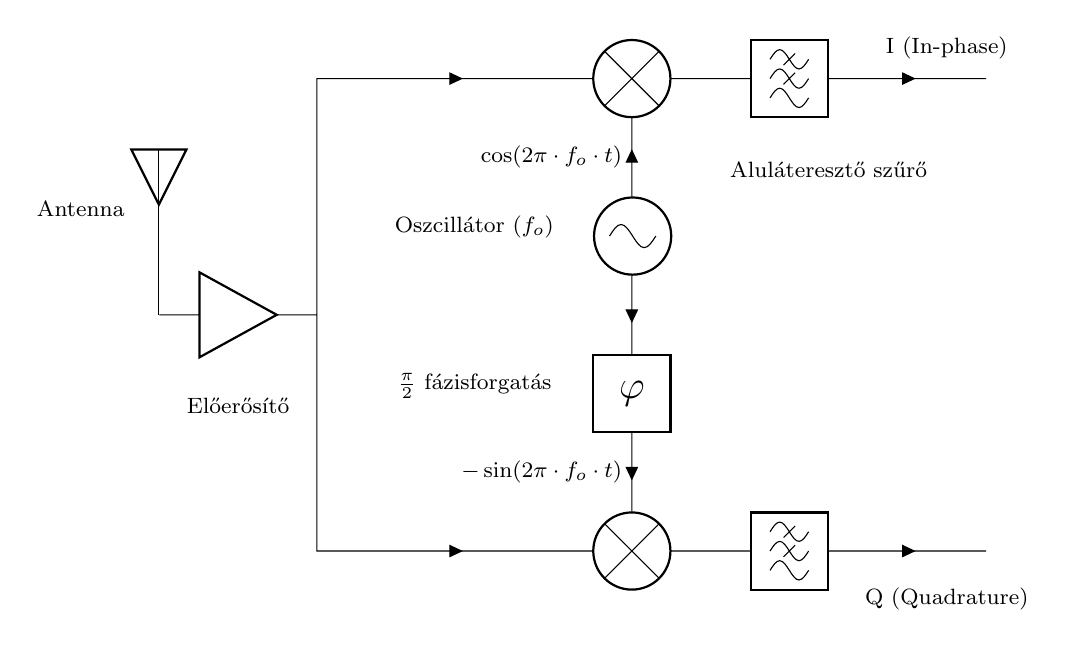
\begin{tikzpicture}

	\draw
	(-1,-2) node[label={[font=\footnotesize]above:Antenna}] {}
	(1,-4.5) node[label={[font=\footnotesize]above:Előerősítő}] {}
	(4,-1.5) node[label={[font=\footnotesize]below:Oszcillátor ($f_o$)}] {}
	(4,-3.5) node[label={[font=\footnotesize]below:$\frac{\pi}{2}$ fázisforgatás}] {}
	
	(8.5,-1.5) node[label={[font=\footnotesize]above:Aluláteresztő szűrő}] {}
	(10,0) node[label={[font=\footnotesize]above:I (In-phase)}] {}
	(10,-7) node[label={[font=\footnotesize]above:Q (Quadrature)}] {}
	
	%(0, -3) to [short] ++(1,0) 
	(2,-3) to [short] ++(0,3) to [short, i=\phantom{}] ++(3.5,0) 
	(2,-3) to [short] ++(0,-3) to [short, i=\phantom{}] ++(3.5,0) 	
	
	(6,-1.5) to [short, i=\footnotesize $\cos(2\pi \cdot f_o \cdot t)$] (6,-0.5)
	
	(6,-2.5) to [short, i=\phantom{}] (6,-3.5)
	
	(6,-4.5) to [short, i>_=\footnotesize $-\sin(2\pi \cdot f_o \cdot t)$] (6,-5.5)
	
	(6.5,0) to [short] ++(1,0) to [lowpass] ++(1,0) to [short, i=\phantom{}] ++(2,0) 
	(6.5,-6) to [short] ++(1,0) to [lowpass] ++(1,0) to [short, i=\phantom{}] ++(2,0) 
	(0, -3) to [amp] ++(2,0) 
	(6,0)[mixer] node(mixa){}	
	(6,-6)[mixer] node(mixb){}	
	

	(0,-3)[antenna]node(ant){}
	(6.5,-2)[oscillator] node(osc){}	
	(6,-4)[phaseshiftershape] node(phas){}	
	
	
	;
    \end{tikzpicture}
\caption{
Az IQ demodulátor egyszerűsített blokkvázlata} 
\end{figure}

\subsection{Komplex jelek}

A komplex jelek szoftveres feldolgozása gyakran könnyebb, mint a csak valós számokból állóké.
Az eredeti vett jel szinuszos komponensei komplex szinuszoidként jelennek meg.

A komplex szinuszoidok a következő alakot veszik fel:
\[
  A e^{j(\phi +  2 \pi f t)} = A ( \cos (\phi + 2 \pi f t)  +  j \sin (\phi + 2 \pi f t))
\]
Az IQ vektorokat ábrázolva ezeket $A$ hosszúságú $f$ frekvenciával az origó körül körbeforgó vektorokként fogjuk látni.
$A$ arányos a jel amplitudójával, $f$ pedig a helyi oszcillátor és a vett komponens frekvenciája közötti eltérés.

Amennyiben a vizsgált komponens frekvenciája nagyobb volt, mint a helyi oszcillátoré, $f$ pozitív lesz, tehát az IQ vektor
az óramutató járásával ellentétesen forog.
Ha a vizsgált komponens frekvenciája kisebb volt, mint a helyi oszcillátoré, $f$ negatív lesz, tehát az IQ vektor
az óramutató járásával megegyezően forog.

Ha az LO és a vett komponens frekvenciája megegyezik, $f = 0$ lesz, így a demodulált IQ vektor konstans.
Ilyenkor $\phi$ az LO és a vett jel közötti fáziseltérés.
(Általánosságban a $\phi + 2\pi ft$ kifejezés értelmezhető a két jel fáziseltéréseként, azonban ez időben változó, ha azok nem azonos frekvenciájúak.)


\subsection{Frekvencia moduláció}

Frekvencia modulációnál egy vivő jel frekvenciájába kódoljuk az $x_m(t)$ moduláló jel által hordozott információt. Az $y(t)$ modulált jelünket a következő képpen számolhatjuk ki:
\[
  y(t) = A \cos(2 \pi t ( f_c + f_{\Delta} x(t) ) )
\]
Itt $A$ az amplitúdónk, $f_c$ a középfrekvenciánk, ez a "vivő eredeti frekvenciája", illetve az állomás névleges frekvenciája (pl. 97.1 MHz). 
$f_{\Delta}$ a frekvencialöket, $\pm 1$ közé normált moduláló jelnél az kimeneti jel energiájának nagy része $f_c \pm f_{\Delta}$ közé esik.

\clearpage
\section{Feladatok}

\subsection{FM demoduláció}

A feladathoz egy RTL-SDR hardvert fogunk felhasználni.
Az USB stick a digitalizált IQ jelet egy bytestreamként küldi: egy 1 byte-os I majd egy 1 byte-os Q mintát küld felváltva.
A 8 bites minták offszettel ábrázolják a negatív értékeket (így például a jel $0$ értékét valójában a $127$-es bináris érték jelenti).
A bytestreamet a demoduláló programunk a standard inputon fogja megkapni, majd a standard outra kell, hogy kiadja az abból kiszámolt hangmintát.

Segítségképpen a minta beolvasás, illetve kiírás már szerepel a kiinduló kódban.
A fogadott IQ jel magasabb mintavételi rátával fog jönni, mint amit a hangkártya kezelni tud, azonban ezt egy külső programmal a demoduláció után fogjuk csökkenteni.
Ezért minden fogadott IQ mintára pontosan egy hangmintát kell a programnak kiadni.

\begin{lstlisting}[frame=single,language=c,caption=Kiinduló kód]
#include <math.h>
#include <stdio.h>

int main()
{
	double i, q, s;
	for(;;) //vegtelen ciklus
	{
                // beolvassuk az I mintat, az offszetet levonjuk, hogy a 0 tenyleg 0 legyen
		i=((unsigned char)getchar()-127); 
                // Q-val ugyan ez
		q=((unsigned char)getchar()-127); //bolvassuk
	
                // s-be kell kiszamolni a demodulalt hangot
                // a kiiras miatt s-t ugy kell skalazni hogy kb. -127 es 128 koze essen.
		// s = ??;

                // s-t visszaalakitjuk offszetese majd kiirjuk
		putchar((unsigned char)(s+127));
	}
}
\end{lstlisting}

\clearpage
A programot saját hardverrel a következő parancssorral lehet futtatni:
\begin{lstlisting}[frame=single,language=bash]
 rtl_sdr -s 240000 -f 89500000 -g 20 - | tcc -lm -run minidemod-wfm.c | sox -t raw -r 240000 -e unsigned -b 8 -c 1 - -t raw - rate 48000 | aplay -f U8 -c1 -r 48000 --buffer-size=200000
\end{lstlisting}

Ha nincs saját hardvered, használhatod a Kafu \texttt{rtl\_mus} szerverét ezzel a paranccsal:
\begin{lstlisting}[frame=single,language=bash]
nc teto.sch.bme.hu 7373 | tcc -lm -run minidemod-wfm.c | sox -t raw -r 240000 -e unsigned -b 8 -c 1 - -t raw - rate 48000 | aplay -f U8 -c1 -r 48000 --buffer-size=200000
\end{lstlisting}

Mindkét parancssorban az egyes programokat a \texttt{|} (pipe) karakter választja el, ami azt jelzi a shellnek,
hogy a balra lévő program standard outját adja át a jobbra lévő program standard injére.

Az \texttt{rtl\_sdr} program az USB stickről olvas mintákat, amiket a standard outra ír. A -s kapcsoló a mintavételi rátát, a -f a helyi oszcillátor frekvenciáját, a -g pedig az erősítést állítja.
Az \texttt{nc} (netcat) egy TCP kapcsolatot hoz létre a megadott szerverrel a megadott porton, és az onnan jövő adatot a standard outra írja.
A megadott gépen és porton egy \texttt{rtl\_mus} nevű program fut, ami a szerverbe dugott RTL-SDRből jövő mintákat fogja továbbítani.

A \texttt{tcc} lefordítja a C kódunkat, és egyből futtatja is az elkészült programot.
A \texttt{sox} az újramintavételezést végzi el, a 240 kHz-s jelből 48 kHz-eset csinál.
Az \texttt{aplay} pedig kijátsza a kapott mintákat a hangkártyán.



\end{document}



